\documentclass[9pt]{beamer}

\mode<presentation> {\usetheme{Kaiping}}
\setbeamercovered{transparent} 

\usepackage[ngerman]{babel}

\usepackage{fontspec}
%\setmainfont{Linux Biolinum}
\setmonofont{DejaVu Sans Mono}
%\setsansfont{Linux Biolinum}

\usepackage{xcolor}
\usepackage{graphicx}
\usepackage{tikz}
\usepackage{tikz-cd}

\usefonttheme[onlymath]{serif}
\usetheme{Warsaw}
% default
% Boadilla
% Madrid
% Pittsburgh
% Rochester \usetheme[height=7mm]{Rochester}
% Copenhagen
% Warsaw
% Singapore
% Malmoe

% Decrease footnote size

\title{Growing Trees from Big Data}
\subtitle{Bayesian Phyologeny for Historical Linguistics}
\author{Gereon Kaiping}
%\institute{Leiden University Centre for Linguistics, the Netherlands}
\date{20-3-2017}

\begin{document}

\begin{frame}[plain]
  \titlepage
\end{frame}
\begin{frame}
  \tableofcontents
\end{frame}
\section{Solutions to All Your Problems!}
\subsection{Crunching Numbers}
\begin{frame}{Problem}
  Using the comparative method is hard, because
  \begin{itemize}
  \item it is a lot of painstaking work,
  \item we don't know how to weigh the evidence,
  \item cognates may have changed meanings,
  \item loan words make our lives more difficult.
  \end{itemize}
  \pause
  And then doesn't even give us dates, just “not before” or “not after” if we are lucky.
\end{frame}
\begin{frame}{Solution}
  Tree reconstruction methods from \textbf{Bioinformatics}
  
  \begin{tikzpicture}
    \uncover<2->{{\node [align=left,anchor=east] (arrow) at (0,0) {→};}}
    \visible<-2>{\uncover<2>{{\node [align=left,anchor=east,font={\scshape\ttfamily}] at (arrow.west) {
      cctccacgcc aacggagcct cattcttctt\\
      cctccacgcc aacaaagcct cattctt---\\
      cctccacgcc aacaaagcct cattcttctt\\
      cctccacgcc aacggagcct caggtgtctt\\
      cctccactcc aacggagcct caggtgtctt};}}}
    \visible<3->{{\node [align=left,anchor=east,red,font={\ttfamily}] at (arrow.west) {
      h ʊ n - ə ɹ - t \_ v ɔ~ ɹ - t\\
      h ʊ n d ɐ - - t \_ β ɔː - - t\\
      h ʊ n d ə - - t \_ β œ~ - - t\\
      h ɐ n d - ɹ ə d \_ w ɜː - - d\\
      h ʊ n d - ɾ a - \_ - oː - - d
      };}}
    \visible<2->{{\node [anchor=west,inner sep=0] (image) at (0,0) {\includegraphics[width=0.5\textwidth,trim={0 0 7cm 0},clip]{Bayesian-Rallus.png}};}}
    \visible<3->{{\node [align=right,red,font={\Huge\bfseries}] at (image.center)
        {Flemish\\Dutch\\German\\Frisian\\English\\Swedish\\Danish\\Norwegian};}}
  \end{tikzpicture}
\end{frame}
\subsection{Bayesian …}
\begin{frame}{Bayes' Theorem}
  \textbf{Bayesian Phylogenetic Inference}, from biology
  
  \textit{Idea:} Evolution = a random process on a tree. What trees are compatible?

  \pause
  Probabilities = confidence of belief, not repeatable random experiment.

  \pause
  “What are consistent beliefs?” = “What trees are consistent with what I believe about evolution?” = “Which histories are likely?”
  \begin{align}
    P(\text{Model} \mid \text{Data}) \propto P(\text{Data} \mid \text{Model}) \times P(\text{Model})
  \end{align}
  \begin{columns}
    \begin{column}{0.5\textwidth}
      \begin{center}
        \includegraphics[width=0.6\textwidth]{scale.png}
      \end{center}
    \end{column}
    \begin{column}{0.5\textwidth}
      \pause
      Bayesian inference is complicated, but
      \begin{itemize}
      \item model-based
      \item can incorporate prior knowledge
      \item outputs result uncertainty
      \end{itemize}
    \end{column}
  \end{columns}
\end{frame}
\subsection{… Phylogenetics}
\begin{frame}{Computational Phylogenetics}
  “Roll dice to generate trees, but only keep the good trees”

  \pause
  Need:
  \begin{itemize}
  \item simple stochastic model(s) of language evolution, with parameters
  \item intuition (“prior”) of how parameters look like
  \item large dataset of model-compatible data
  \end{itemize}

  \pause
  Data:
  \begin{itemize}
  \item Swadesh lists: models going back to Glottochronology – but better
  \item Geography: various models
  \item Phonetic word lists: still in infancy
  \item Typological data: Some approaches, problems with universals/pathways
  \item Morphosyntax: ??????
  \end{itemize}
\end{frame}
\section{[Examples]}
\subsection{Austronesian: Branches and times}
\begin{frame}{Example 1: Austronesian}
  \begin{columns}
    \begin{column}{0.5\textwidth}
      \includegraphics[page=1,width=\textwidth]{abvd-hand.pdf}
    \end{column}
    \begin{column}{0.5\textwidth}
      \begin{itemize}
      \item Austronesian Basic Vocabulary Database: several 1000 cognate classes for 210 meanings in 400 langs
      \item Plus two “outgroup” langs, minus borrowings
      \item Binary covarion model
      \item Calibrations and variable replacement rates
      \end{itemize}
    \end{column}
  \end{columns}
\end{frame}
\begin{frame}{Example 1: Austronesian}
  \begin{columns}
    \begin{column}{0.5\textwidth}
      \includegraphics[width=\textwidth,page=2,trim={2cm 4cm 1cm 5cm},clip]{austronesian.pdf}
    \end{column}
    \begin{column}{0.5\textwidth}
      \footnotesize “The invention of the outrigger canoe and its
        sail may have enabled the Austronesians to move across this
        channel before spreading rapidly over the 7000 km from the
        Philippines to Polynesia (4). This is supported by linguistic
        reconstructions showing that the terminology associated with
        the outrigger canoe complex can only be traced back to Proto-
        Malayo-Polynesian and not Proto-Austronesian (41).”
      \includegraphics[width=0.8\textwidth,page=3,trim={1cm 1cm 7.5cm 16cm},clip]{austronesian.pdf}
    \end{column}
  \end{columns}
\end{frame}
\subsection{Bantu: Phylogeography}
\begin{frame}{Example 2: Bantu}
  \begin{columns}
    \begin{column}{0.5\textwidth}
      \begin{itemize}
      \item 2908 cognate classes for 90 meanings in 542 varieties of Bantu/Bantoid,
        with geographical point-coordinates
      \item Binary covarion with 6 (empir.) rate categories
      \item Brownian motion ancestral state reconstruction of
        latitudes and longitudes on 500 best trees
      \item Other statistical analyses
      \end{itemize}
    \end{column}
    \begin{column}{0.5\textwidth}
    \end{column}
  \end{columns}
\end{frame}
\begin{frame}{Example 2: Bantu}
  \begin{columns}
    \begin{column}{0.5\textwidth}
      \includegraphics[width=\textwidth,page=5,trim={5cm 11.5cm 3cm 1cm},clip]{bantu.pdf}
    \end{column}
    \begin{column}{0.5\textwidth}
      \footnotesize “These debates have implications regarding the
      origin and spread of important cultural innovations, such as
      metallurgy and cattle-keeping.”

      “[…] explicit mapping of ancestral locations to make
      inferences about the specific route taken during the dispersal
      of Bantu languages. The results clearly support the ‘pathway
      through the rainforest’ scenario for the expansion of Bantu
      through much of sub-Saharan Africa. There is no support
      in these analyses for an early, deep split between East and
      West Bantu languages and a movement by one branch
      north of the rainforest.”
    \end{column}
  \end{columns}
\end{frame}
\section{And why actually not.}
\begin{frame}{Criticism}
  Some papers
  \begin{itemize}
  \item disregard prior knowledge
  \item use models that don't fit their data
  \end{itemize}
  \pause
  State of the art models
  \begin{itemize}
  \item can only build trees, no language contact
  \item only support cognate data (baby steps towards phonetic data and typology)
  \item are not realistic and not calibrated
  \end{itemize}
  \pause
  We might never
  \begin{itemize}
  \item properly model morphosyntax
  \end{itemize}
\end{frame}
\section{Conclusions}
\begin{frame}{Conclusions}
  \begin{itemize}
  \item Computer models can help make sense of large data sets
  \item Mathematical models can handle new \emph{types} of data for new types of results
  \item Very few language-specific models so far
  \item If you disagree with results, \emph{what parameters or choices do you disagree with?}
  \end{itemize}
\end{frame}
\subsection{Further Reading}
\begin{frame}
  Course
  Literature: McMahon \& McMahon
\end{frame}
\end{document}
%%% Local Variables:
%%% TeX-engine: luatex
%%% End: 
